% Auto-generated publication figure environments (paths are repository-relative).
\begin{figure}[t]
  \centering
  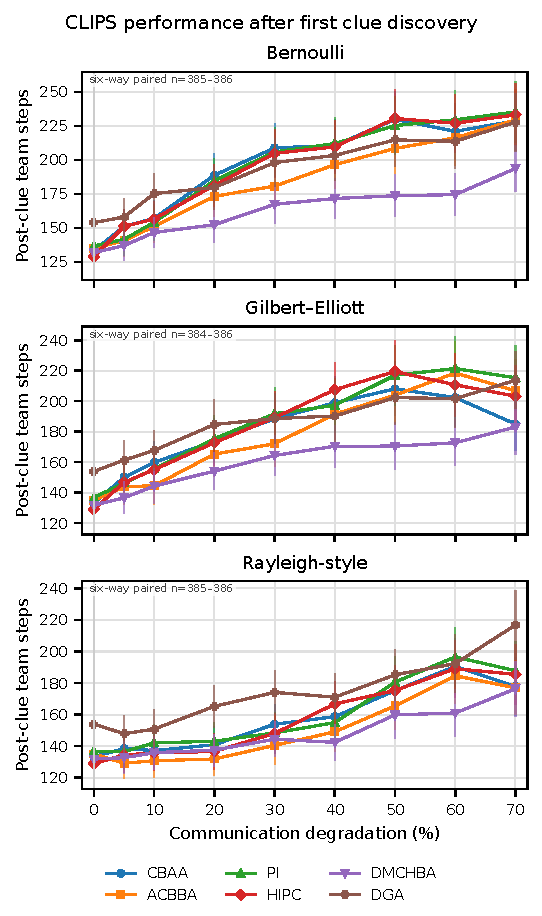
\includegraphics[width=\columnwidth]{results/analysis/figures/clips_post_clue_steps_final.pdf}
  \caption{Clue-Informed Probabilistic Search (CLIPS) performance after first clue discovery. Points are six-algorithm-paired means of \texttt{post\_clue\_steps\_to\_find}; vertical intervals are 95\% Student-$t$ confidence intervals. Each panel reports the paired sample-size range, and the ideal point is repeated at 0\% only as a common baseline. Source: \texttt{figure\_clips\_post\_clue\_source.csv}.}
  \label{fig:clips-post-clue}
\end{figure}

\begin{figure*}[t]
  \centering
  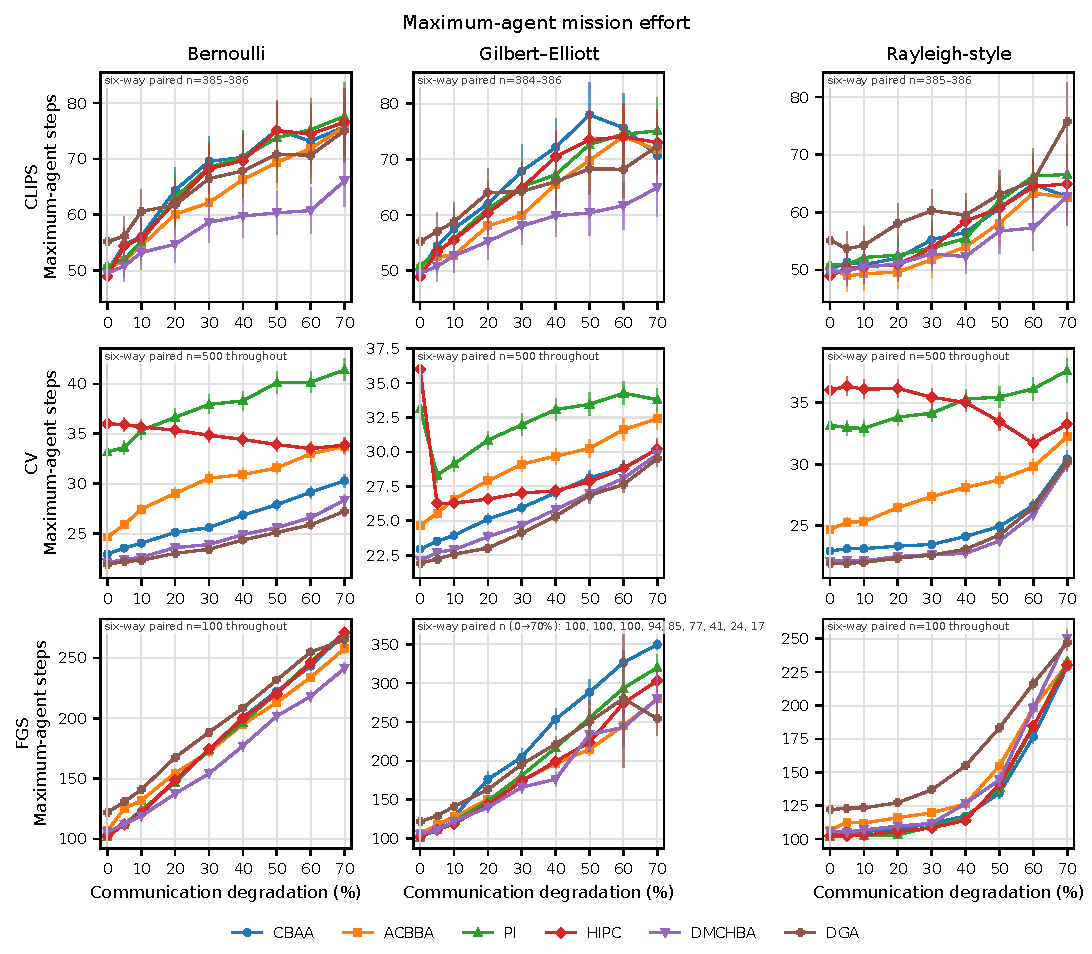
\includegraphics[width=\textwidth]{results/analysis/figures/max_agent_steps_all_missions_final.pdf}
  \caption{Maximum-agent steps for CLIPS, Collaborative Visit (CV), and Full Grid Search (FGS), separated by communication model. Points are six-algorithm-paired means with 95\% Student-$t$ confidence intervals. Printed $n$ values expose the declining conditional-on-completion support for FGS under severe Gilbert--Elliott loss. Source: \texttt{figure\_maximum\_agent\_steps\_source.csv}.}
  \label{fig:maximum-agent-steps}
\end{figure*}

\begin{figure}[t]
  \centering
  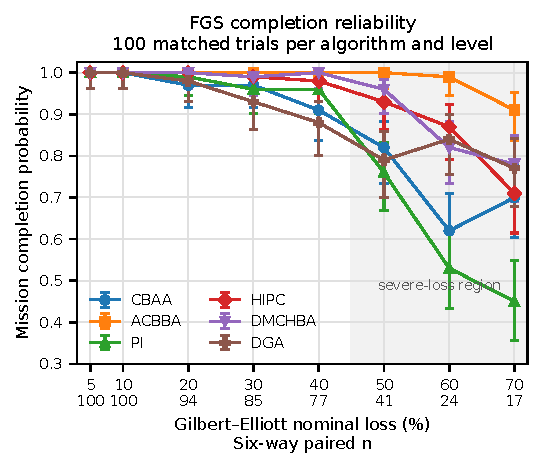
\includegraphics[width=\columnwidth]{results/analysis/figures/fgs_completion_rates_final.pdf}
  \caption{FGS mission-completion probability under the corrected Gilbert--Elliott process. Points show completion proportions over 100 matched trials per algorithm at each nominal loss level, and error bars are 95\% Wilson intervals. The second row of horizontal-axis labels reports the number of trial IDs completed by all six algorithms and therefore available for conditional continuous-metric comparison. Source: \texttt{figure\_fgs\_completion\_source.csv}.}
  \label{fig:fgs-completion}
\end{figure}

\begin{figure*}[t]
  \centering
  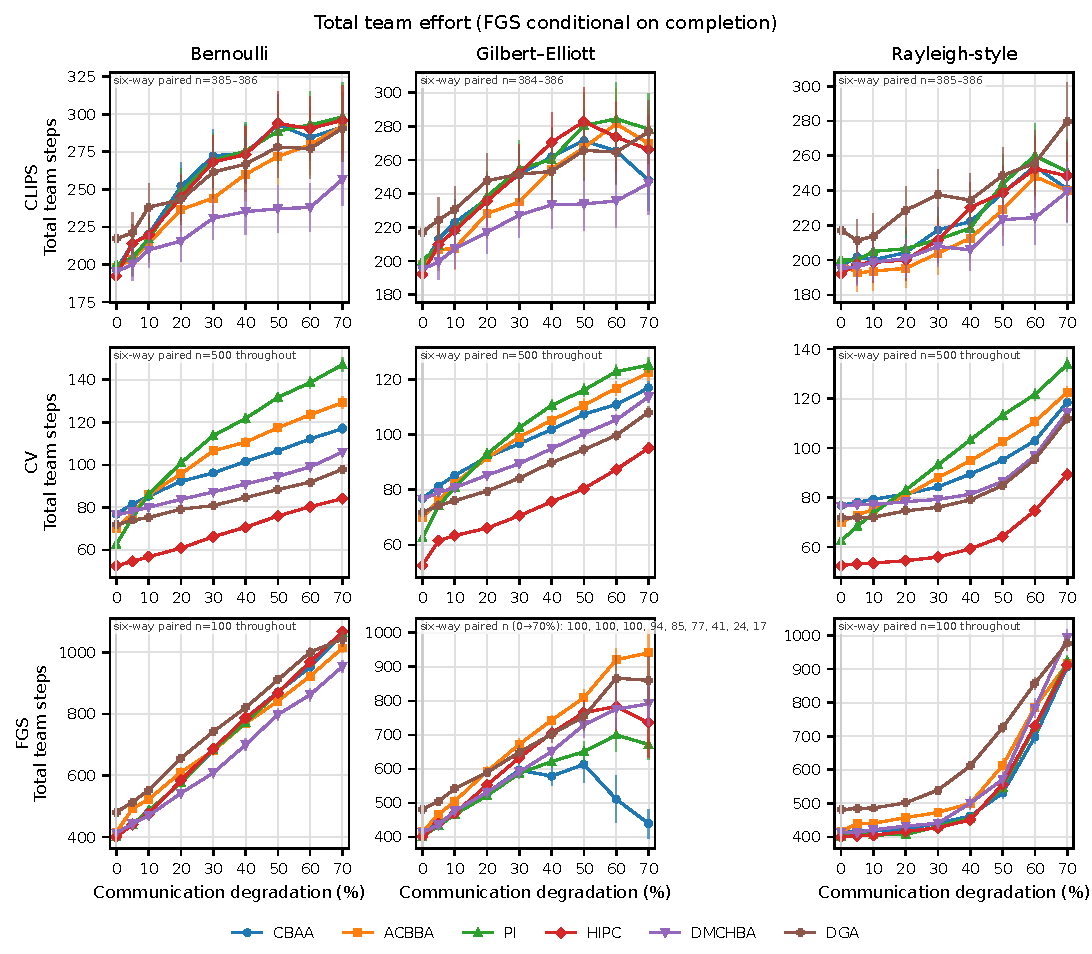
\includegraphics[width=\textwidth]{results/analysis/figures/total_team_steps.pdf}
  \caption{Total team steps by mission and communication model. Intervals represent trial uncertainty (95\% Student-$t$ confidence intervals), not ranges across degradation levels. FGS values are explicitly conditional on successful completion and use the printed six-way-paired $n$. Source: \texttt{figure\_total\_team\_steps\_source.csv}.}
  \label{fig:total-team-steps}
\end{figure*}

\begin{figure}[t]
  \centering
  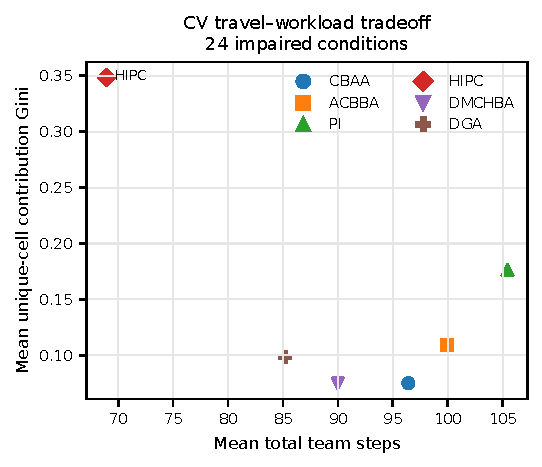
\includegraphics[width=\columnwidth]{results/analysis/figures/cv_workload_tradeoff.pdf}
  \caption{CV aggregate-travel--workload tradeoff across the 24 impaired conditions. Points show each algorithm's unweighted mean total team steps and mean unique-cell contribution Gini; the lower-left region is preferred when both total motion and workload balance matter. HIPC minimizes aggregate travel but concentrates substantially more work on a subset of robots. Source: \texttt{figure\_cv\_workload\_tradeoff\_source.csv}.}
  \label{fig:cv-workload-tradeoff}
\end{figure}

\begin{figure*}[t]
  \centering
  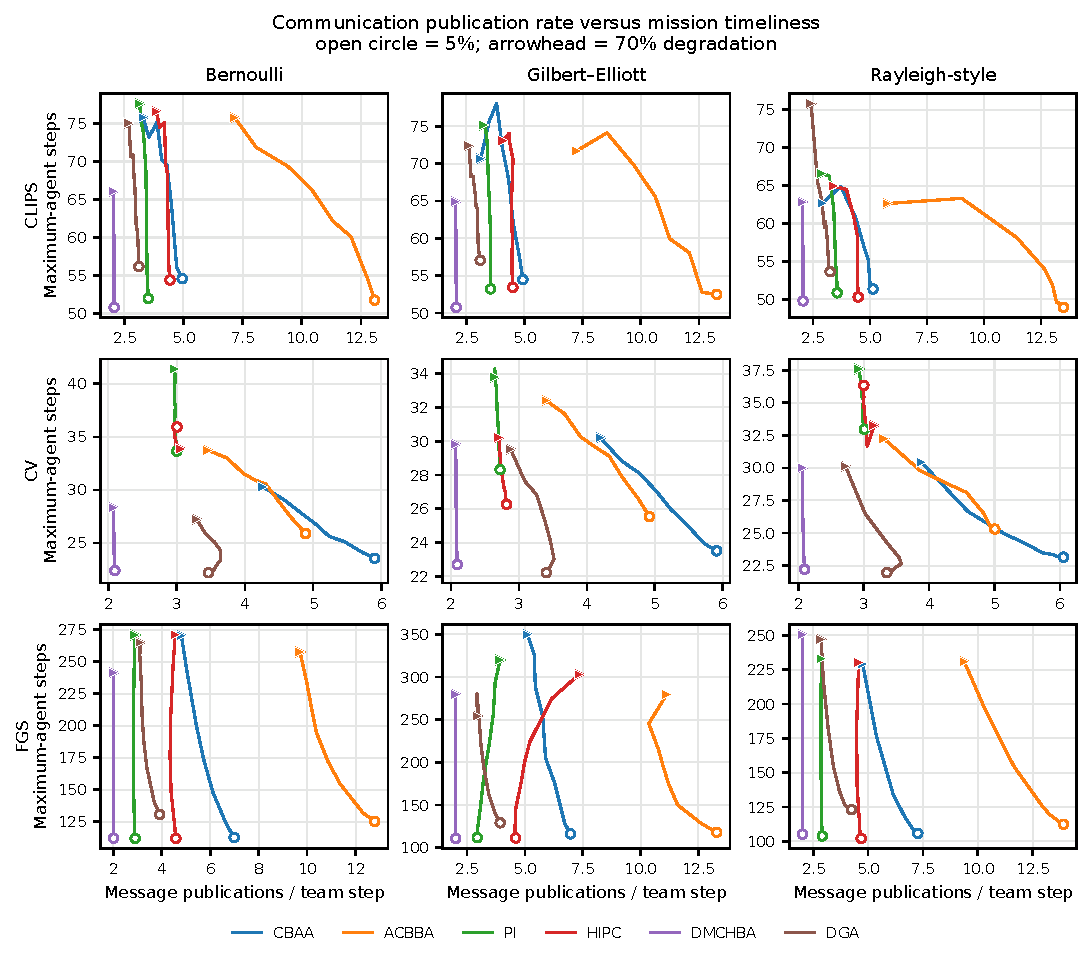
\includegraphics[width=\textwidth]{results/analysis/figures/communication_performance_tradeoff_revised.pdf}
  \caption{Communication--mission tradeoff across CLIPS, CV, and FGS. Each algorithm trajectory relates message publications per team step to absolute maximum-agent steps as nominal degradation increases from 5\% to 70\%. The lower-left region is preferred. Open circles identify 5\% and arrowheads identify 70\%; FGS points are conditional on successful completion. Source: \texttt{figure\_communication\_tradeoff\_source.csv}.}
  \label{fig:communication-tradeoff}
\end{figure*}

\begin{figure*}[t]
  \centering
  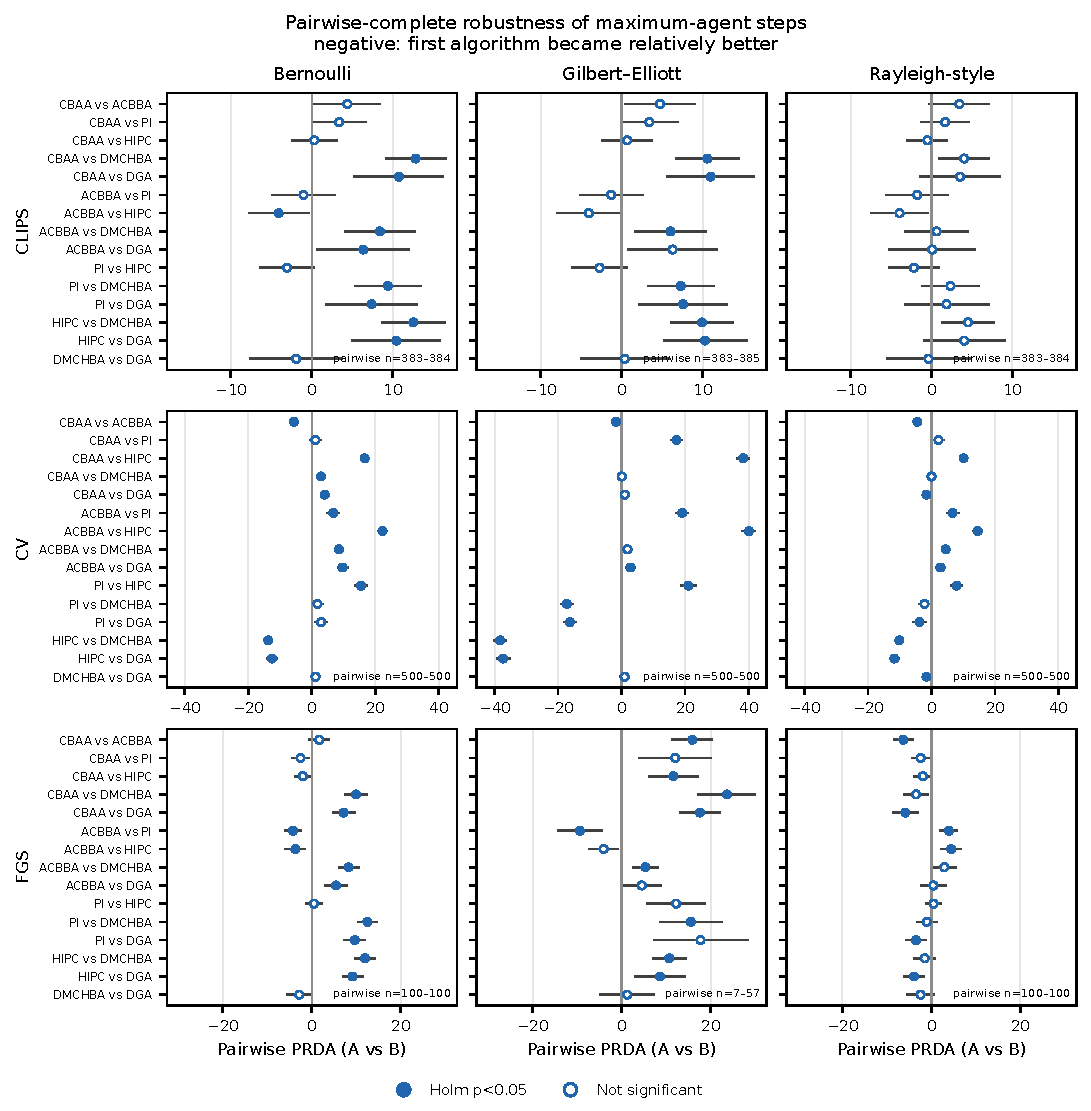
\includegraphics[width=\textwidth]{results/analysis/figures/prda_pairwise_complete_final.pdf}
  \caption{Pairwise-complete relative degradation area (PRDA) for maximum-agent steps, with communication models kept separate. Points show means with 95\% Student-$t$ confidence intervals. Negative values mean the first named algorithm became relatively better as degradation increased. Filled markers denote Holm-adjusted $p<0.05$, open markers denote nonsignificant comparisons, and panel annotations give pairwise-complete $n$ ranges. Source: \texttt{figure\_pairwise\_prda\_source.csv}.}
  \label{fig:pairwise-prda}
\end{figure*}

\begin{figure*}[t]
  \centering
  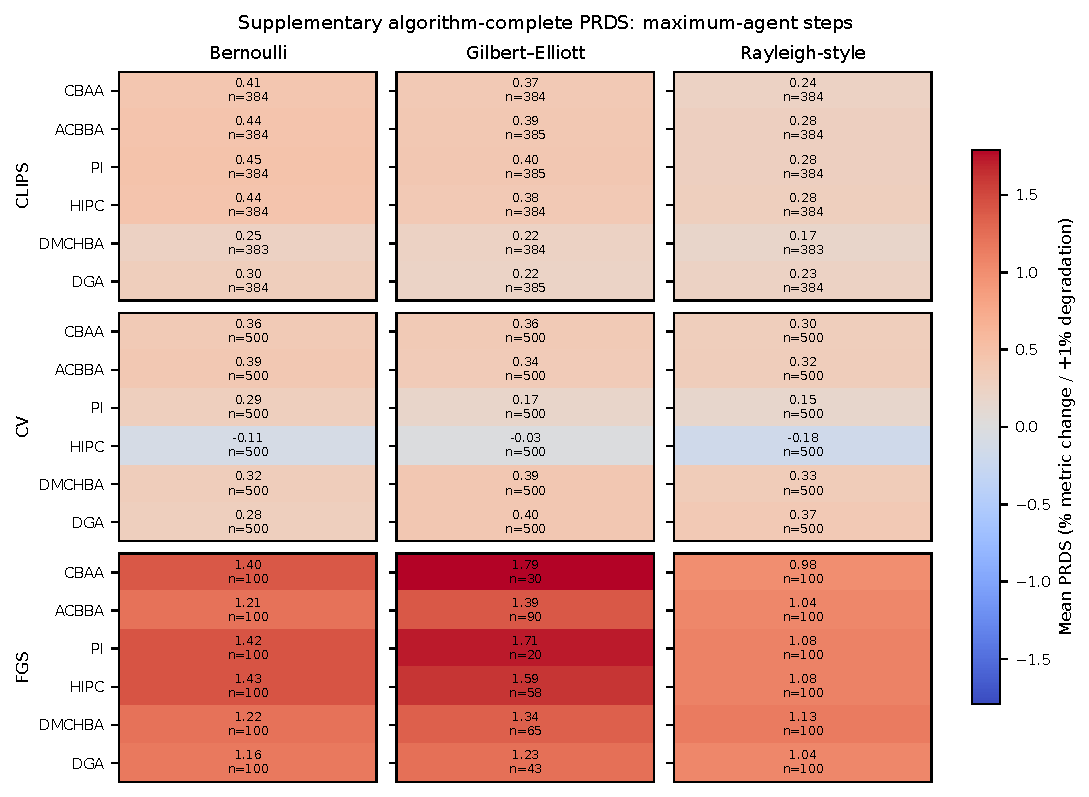
\includegraphics[width=\textwidth]{results/analysis/figures/prds_supplement.pdf}
  \caption{Supplementary algorithm-complete proportional robustness degradation slope (PRDS) for maximum-agent steps. Communication models are not averaged; each cell reports the mean PRDS and eligible algorithm-specific trajectory $n$. Source: \texttt{figure\_prds\_supplement\_source.csv}.}
  \label{fig:prds-supplement}
\end{figure*}

\begin{figure}[t]
  \centering
  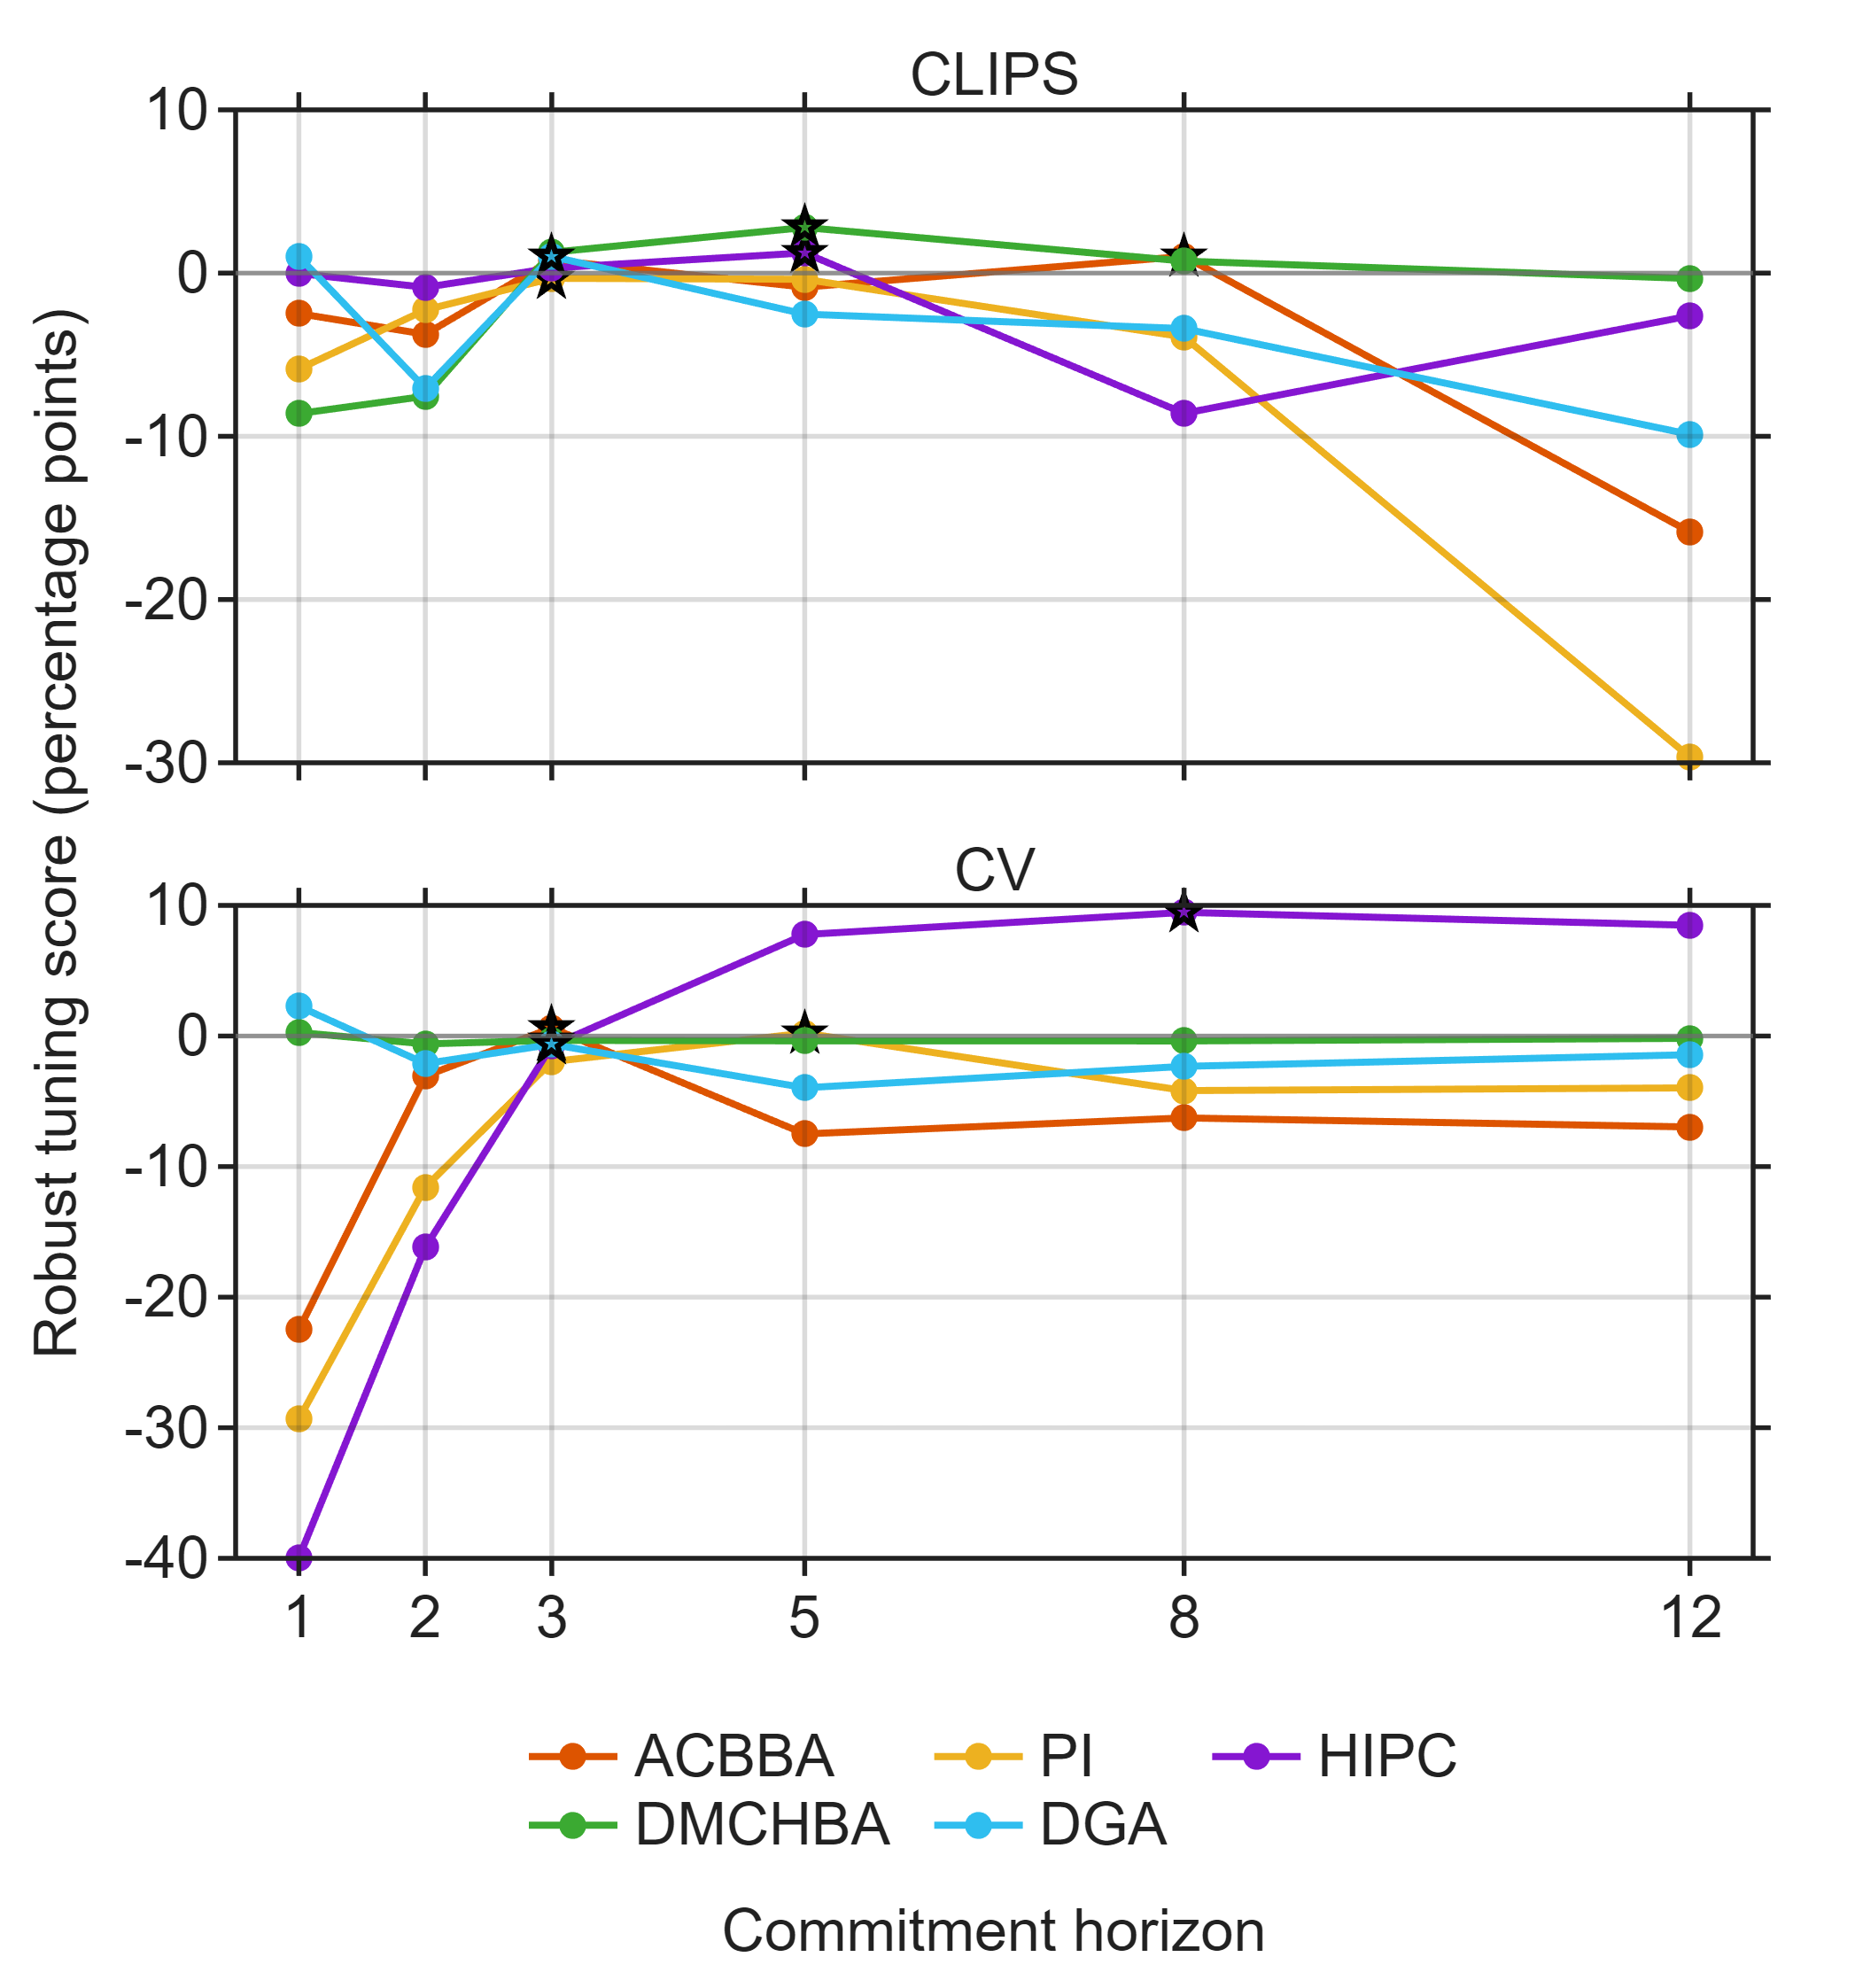
\includegraphics[width=\columnwidth]{results/analysis/figures/horizon_tuning.png}
  \caption{Commitment-horizon sensitivity for CV, CLIPS, and FGS. Within each scenario, algorithm, and trial, the paired baseline is the mean metric over all tested horizons and both communication settings; plotted values are metric-minus-baseline means. Solid lines denote ideal communication, dotted lines Bernoulli loss probability 0.25, and stars mark the selected main-benchmark horizon for each algorithm and mission. Source: \texttt{horizon\_tuning\_paired\_trial\_delta\_summary.csv}.}
  \label{fig:horizon-tuning}
\end{figure}

\begin{figure}[t]
  \centering
  \includegraphics[width=\columnwidth]{results/analysis/figures/DGA_iteration.png}
  \caption{DGA generation-count sensitivity in CV under ideal and Bernoulli $p_d=0.25$ communication. Values are mean percent differences from the per-trial average over all tested DGA iteration counts. Stars mark the main-benchmark value $k=25$. The available sensitivity bundle contains no corresponding CLIPS sweep. Source: \texttt{dga\_iteration\_percent\_delta\_summary.csv}.}
  \label{fig:dga-iteration}
\end{figure}
